\chapter{Related Work}
In this chapter we present work related to this thesis. In section 3.1, we descibe alternatives to Gazebo and why we choose Gazebo. In section 3.2, we give an overview of other popular simulations, especially a simulation that also uses Gazebo and other multi-robot simulations, and in section 3.3, we describe our current multi-robot strategy as well as other attractive strategies our simulation should be able to evaluate. In the following, we will use the terms \textit{multi-robot} and \textit{multi-agent} interchangeably because the common term in litrature is multi-agent and we want to use multi-robot. A multi-agent system can consist of fully abstract agents, such as \textcolor{red}{...}, whereas we are dealing with multi-robot system and therefore robots that interact physically with their environment.


\section{Other Simulators}
\textcolor{red}{blabla?}
\subsection{Stage}
\textit{Stage}\footnote{\url{http://playerstage.sourceforge.net/index.php?src=stage}} is an Open Source multi-robot simulator for a two dimensional environment. It is a part of the \textit{Player/Stage} project~\cite{{PlayerStage}}. \textit{Player} is a robot control server, which provides a simple connection between a robot control program and the sensors and actuators of a robot. Stage uses this connection and replaces the sensors and actuators by simulated ones. Stage was popular simulator in the last years and is able to simulate a large amount of robots. For the simulation, stages simple and computationaly cheap models, that provide still enough fidelity for most applications. Furthermore the computational effort is linear in the number of robots. Because of that, Stage can simulate large amounts of robots~\cite{stage_massive}. This makes Stage attractive for the simulation of swarms and multi-robot systems with many robots.

\subsection{Webots}
\textit{Webots}\footnote{\url{http://www.cyberbotics.com}} is a commercial 3D-simulator~\cite{{Webots}}. It is platform independent features a whole development environment for robot software including an editor and an \textcolor{red}{API} for inter-robot communication. Webots supports many programming languages and supports a variat of standard robots and sensors out of the box. It is also able to simulate multiple robots and provides a ROS and \textcolor{red}{Matlab} interface.\\
Webots was used in a RoboCup Soccer simulation league~\cite{webots_robocup}.

\subsection{USARSim}
\textit{USARSim} is a 3D-simulator that was developed for urban search and rescue scenarios~\cite{USARSim}. It was envolved to be able to simulate other domains too. Therefore, the abbriviation USARSim now stands for ``Unified System for Automation 
and Robotics Simulation'' instead of te previous ``Urban Search and Rescue Simulation''~\cite{usarsim_new}. It is platform independent and free of charge for research and education. It's advantages are the graphical quality of the Unreal engine\footnote{\url{http://www.unrealengine.com/udk}} and the PhysX physics engine\footnote{\url{https://developer.nvidia.com/physx}}. USARSim also provides an interface to ROS~\cite{USARSimROS} and is able to simulate multiple robots.\\
USARSim is used as a basis for the RoboCup Rescue Simulation League we also present in section 3.2.2.

\subsection{SimSpark}
\textit{SimSpark}\footnote{\url{http://simspark.sourceforge.net/}} is an Open Source 3D simulator~\cite{simspark_old}. It was developed by the RoboCup community for the RoboCup 3D Soccer Simulation and has been used there since 2004. Therefore SimSpark is able to simulate multiple robots and specialised on the NAO as soccer robot. There are several improvementsand new features of SimSpark~\cite{SimSpark,Visualization}, such as visualization of agent-intentions, realistic servo motors for the NAO and better support of heterogenous robot teams.

\subsection{Robotino Sim Professional}
\textit{Robotino Sim Professional}\footnote{\url{http://www.festo-didactic.com/int-en/learning-systems/software-e-learning/robotino-sim-view/robotino-sim-professional.htm}} is a 3D-simulator for the Robotino developed by its manufacturer Festo. It is a commercial software and only usable on Microsoft Windows. Furthermore, it is limited to the Robotino and the default sensors the robotino is sold with.

\subsection{Choice for Gazebo}
We aready presented Gazebo and some of its advantages in section 2.4. Here we explain why we have chosen Gazebo instead of an alternative we described above.\\
The stage simulator is well suited for multi-robot systems and comparatively fast and easy to use. However, the restriction to dimensions is a problem. We want to simulate vision components as well to be able to test our system as a whole and more realistic. We also want to be extendable for future changes of LLSF or the use of the simulator in an other domain, such as the RoboCup @Home league.\\
Webots is a proven simulator with many features, but has the same problems as Robotino Sim Professional. On the one hand both simulators are commercial and on the other hand both are no Open Source software. Therefore it can be difficult to expand the simulation how we need it.\\
SimSpark is not so well suited as Gazebo because it and the community behind are mostly specialized on the RoboCup Soccer Simulation. Gazebo is used in large variaty of domains and has a bigger community. Gazebo is well founded by the Open Source Robotics Foundation\footnote{\url{http://osrfoundation.org/}} and Willow Garage\footnote{\url{http://www.willowgarage.com/}} and there are also many plans to develop Gazebo further\footnote{\textcolor{red}{link roadmap}}. Therefore Gazebo is likely to become even more important in the future.\\
An other important argument for Gazebo is that it was used at KBSG before. It was used as a simulator for MSL~\cite{MultiLevelAbstraction} and it was used for a scene reconstruction~\cite{KlingenDA}. We will present both later in this chapter.\\
There are only few disadvantages of Gazebo for this thesis. A disadvantage is that Gazebo can not handle larger number of robots. The complexity of the simulations limits the simulation speed when using multiple robots. The number of robots to simulate at a reasonable speed is in the order of ten~\cite{GazeboDesign}. This can become a problem if the simulation runs on a slow computer or there are more robots to simulate at the same time.

\section{Simulations}
\textcolor{red}{blabla?}
\subsection{Virtual Robotics Challenge}
The \textit{Virtual Robotics Challenge (VRC)} is a competition by DARPA\footnote{DARPA is the Defense Advanced Research Projects Agency of the USA.}. The goal of the competitin is to solve challenging tasks with a humaniod robot in a simulation. VRC is the first part of the \textit{DARPA Robotics Callenge (DRC)}\footnote{\url{http://www.theroboticschallenge.org/}}. DRC aims to spur the development of robots that can operate in a desaster scenario if the situation is too dangerous for humans. An example for such a scenario is the desaster in the Fukushima nuclear power plant after tsunami in March 2011~\cite{fukushima}. The developed robots should be able to operate in environment made for humans, even if the environment is damaged, and to use tools made for humans, such as screwdrivers and cars. During the competition the robots act partly autonomously and are supervised by a human instructor. For the callenge, DARPA provides six humanoid robots. The Robots are called ATLAS and are developed by Boston Dynamics. The six best teams of VRC receive a ATLAS robot for free. Therefore ATLAS is the only robot simulated in VRC. However the participating teams can also build their own robots. VRC consists of three different tasks~\cite{vrc_rules} showed in Figure~\ref{fig:vrc}.
\begin{figure}
  \centering
  \begin{subfigure}[b]{0.3\textwidth}
    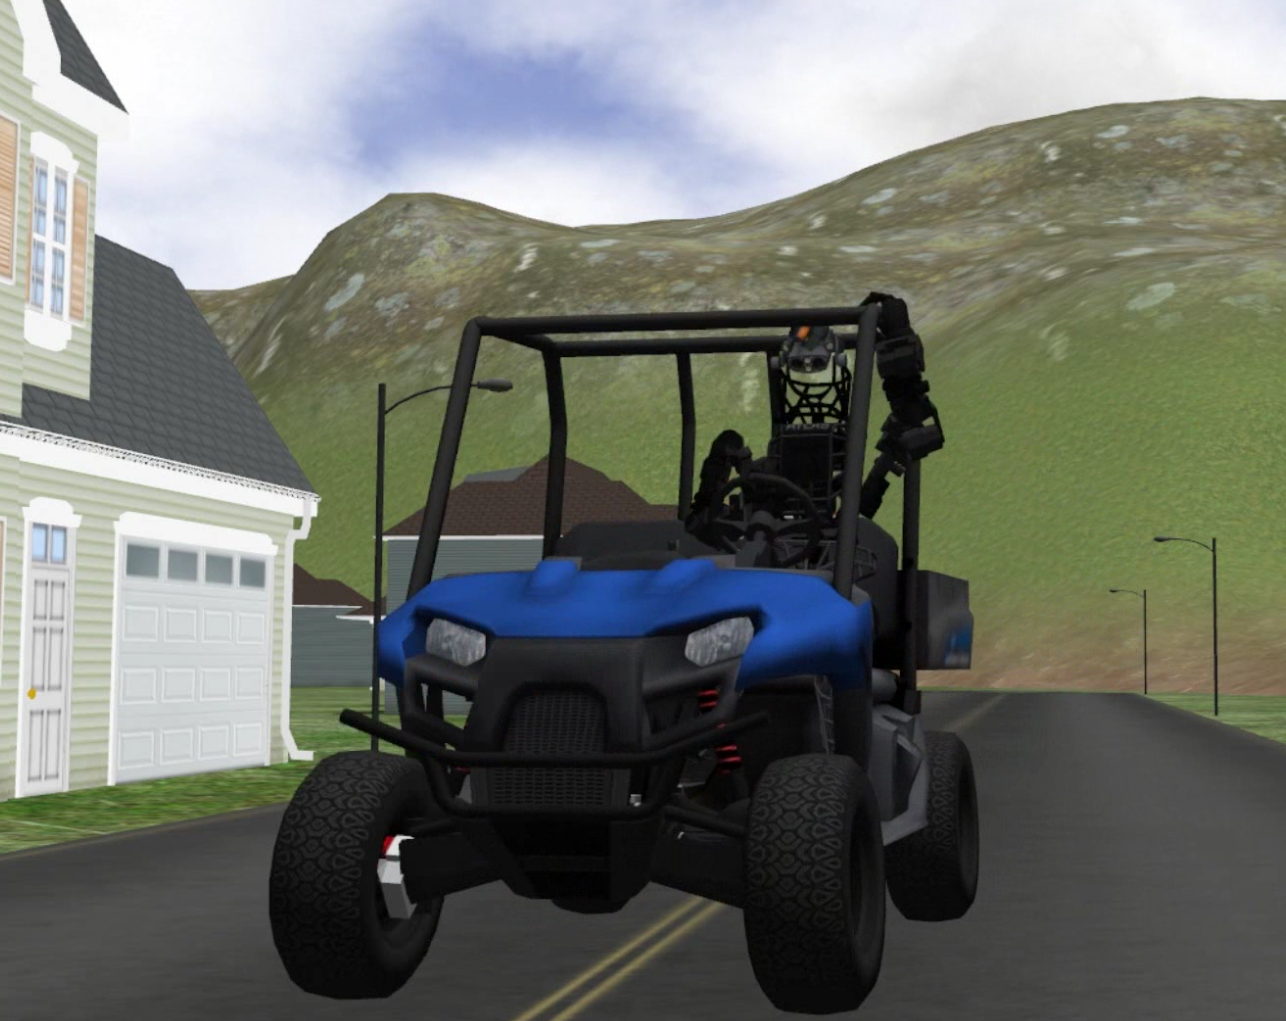
\includegraphics[width=\textwidth]{pics/darpa_car}
    \caption{Driving a car}
    \label{fig:vrc_car}
  \end{subfigure}
  \begin{subfigure}[b]{0.3\textwidth}
    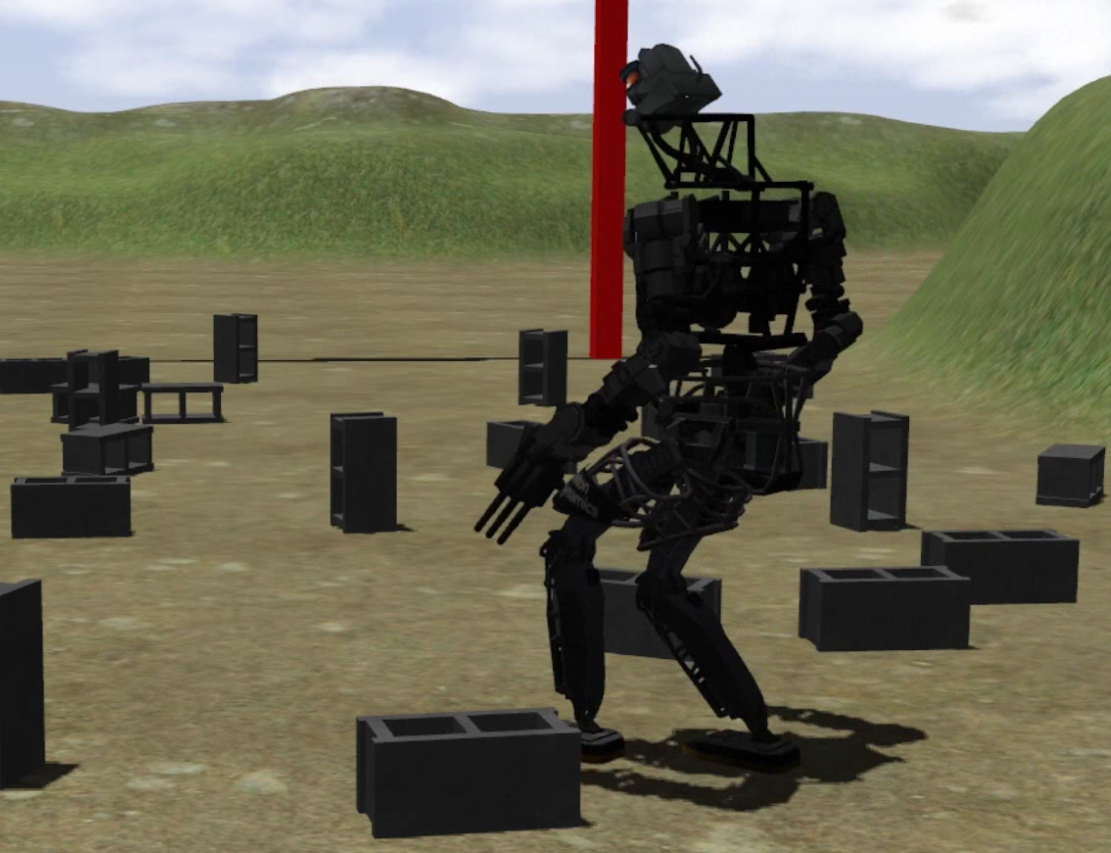
\includegraphics[width=\textwidth]{pics/darpa_walking}
    \caption{Crossing rough terrain}
    \label{fig:vrc_walking}
  \end{subfigure}
  \begin{subfigure}[b]{0.3\textwidth}
    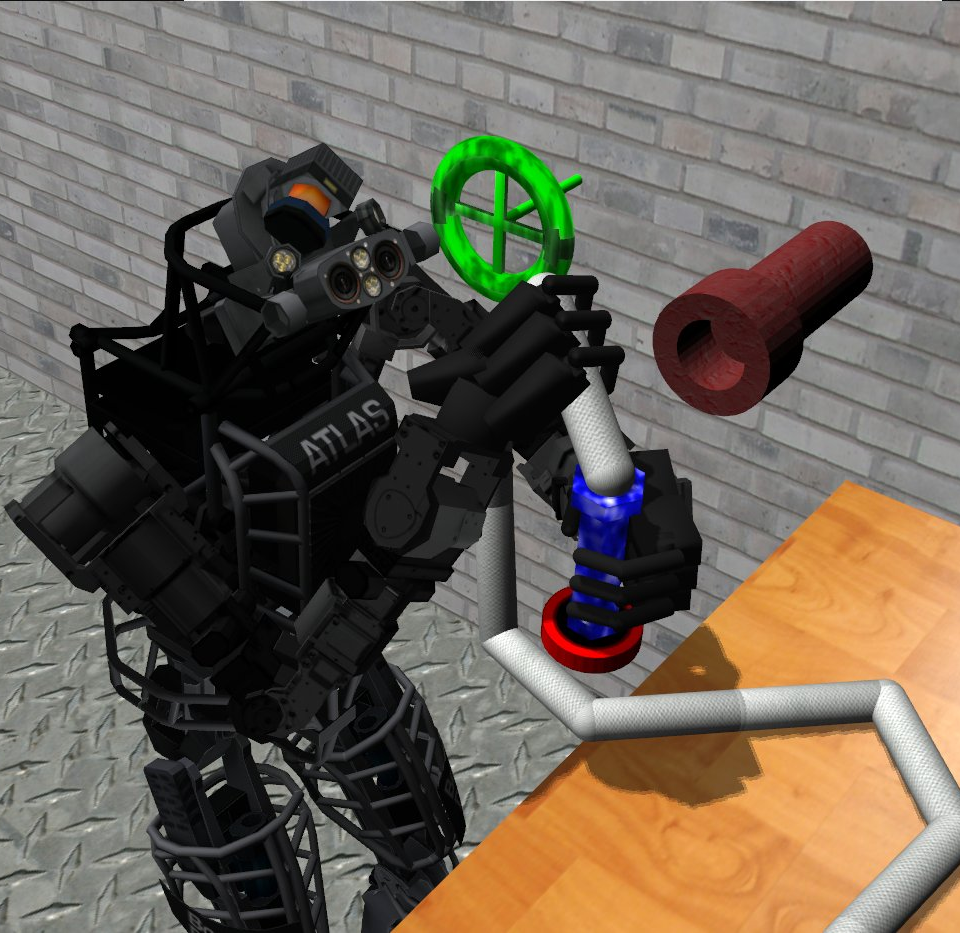
\includegraphics[width=\textwidth]{pics/darpa_hose}
    \caption{Connecting a hose}
    \label{fig:vrc_hose}
  \end{subfigure}
  \caption{Tasks of the Virtual Robotics Challenge~\cite{vrc_pics}}
  \label{fig:vrc}
\end{figure}
In the first task, the robot has to walk to a car, enter it and drive along a street. The chasis of the car consists of a framework to simplify the entry. On the road, there are obstacles the robot has to avoid. The second tasks tests the walking capabilities of the robot. The robot has to cross slippery and irregular terrain to test balancing and a terrain with obstacles to test perception and footstep planning. The last task is about manipulation. The robot has to connect a hose to a pipe by pluggin it in and scrweing it down. Afterwards, it has to open a valve. All tasks have randomized parameters, such as the position of obstacles and goals.\\
VRC is related to this thesis because it also uses the Gazebo simulator~\cite{IEEESpectrum}. Therefore it shows what Gazebo is capabile of and how important a simulation is for the development and research of cutting-edge technology. \textcolor{red}{more}
Altough the technology fostered by DRC is important and useful without doubt, it seems questionable what DARPA as a military agency will use this technology for.


\subsection{RoboCup Simulation Leagues}
In the RoboCup competition, there are different simulation leagues. On the one hand, there are the 2D and 3D soccer simulation leagues and on the other hand, there are two rescue simulation leagues. In all of those leagues, multi-robot coordination is a important field. This is not suprising because it is much simpler to benchmark multi-robot strategies in a simulation. There is no need to operate real hardware and difficult low level control and sense problems, that are not the focus of the benchmark, can be simplified or left out.\\
\begin{figure}
  \centering
  \begin{subfigure}[b]{0.48\textwidth}
    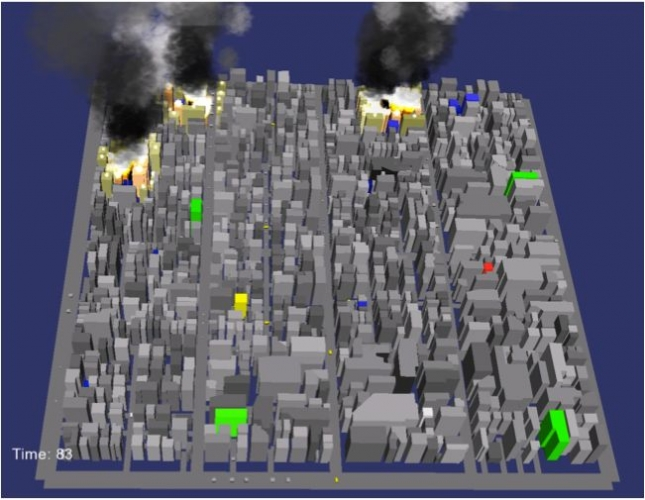
\includegraphics[width=\textwidth]{pics/rescue3d}
    \caption{Agent Competition~\cite{rescue3d}}
    \label{fig:rescue_agent_competition}
  \end{subfigure}
  \begin{subfigure}[b]{0.48\textwidth}
    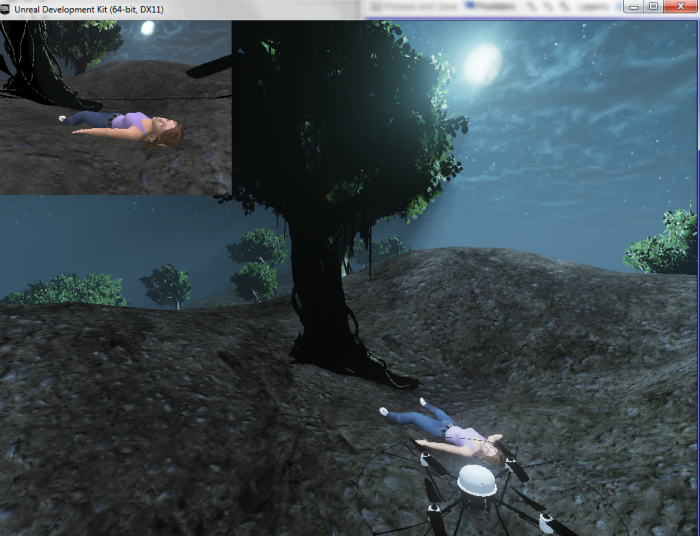
\includegraphics[width=\textwidth]{pics/rescue_vrc}
    \caption{Virtual Robot Competition~\cite{rescue_simulation_league}}
    \label{fig:rescue_vrc}
  \end{subfigure}
  \caption{Rescue Simulation Leagues}
  \label{fig:rescue}
\end{figure}
The \textit{Rescue Simulation League (RSL)} aims to benchmark intelligent software agents and robots in a disaster scenario~\cite{rescue_simulation_league}. RSL is seperated into to leagues with different with focus on different scales. Figure~\ref{fig:rescue} shows snapshots of both simulation. The \textit{Agent Competition} is about a large scale disaster in a city with multiple robot teams. The \textit{Virtual Robot Competition} is about finding victims in a burning house or limited outdoor area with a team of eight robots and one human operator. The operator can give high level commands, such as the area where to look for victims, and is needed to verify the observations of the robots. So, the robots should find and approach victims autonomously and the operator has to confirm it. The task of the agents include victim-detection, autonomous generation of maps, navigation and multi-robot coordination. In the Agent Competition, there is no realistic robot control and perception necessary. The focus is on the coordination of many heterogenous agents to take high level decisions. There are teams of fire brigarde, police and ambulance, each with up to 30 simulated agents. Each agent acts automomously and can communicate with other agents. The tasks of the agents include exploration, scheduling and planning in cooperation with other agents and building of agent teams (e.g. to fight fires more effectively).\\
\begin{figure}
  \centering
  \begin{subfigure}[b]{0.48\textwidth}
    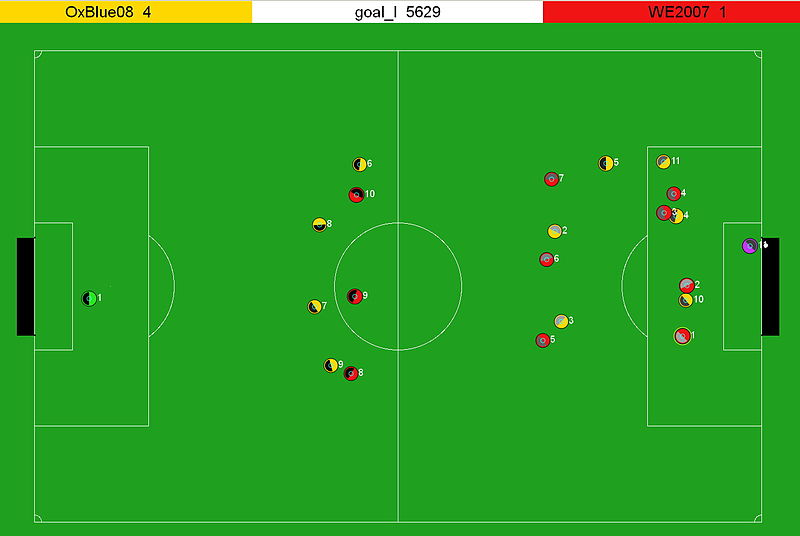
\includegraphics[width=\textwidth]{pics/soccer_simulation_2d}
    \caption{2D Soccer Simulation League~\cite{soccer_simulation_2d_pic}}
    \label{fig:soccer_simulation_2d}
  \end{subfigure}
  \begin{subfigure}[b]{0.48\textwidth}
    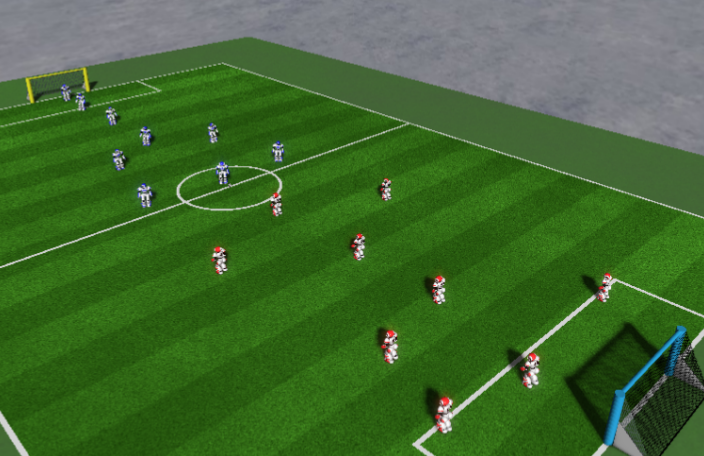
\includegraphics[width=\textwidth]{pics/soccer_simulation_3d}
    \caption{3D Soccer Simulation League~\cite{soccer_simulation_low_level}}
    \label{fig:soccer_simulation_3d}
  \end{subfigure}
  \caption{RoboCup Soccer Simulation Leagues}
  \label{fig:soccer_simulation}
\end{figure}
The soccer simulations of the RoboCup are similary splitted in two leagues. In the \textit{2D Soccer Simulation League}, 22 agents in two teams play soccer in a two dimensional environment. A single server called Soccer Server simulates and controls the game with its physics, the actions of the agents and the perception of the agents. Each agent is an autonomous programm and communicates with the soccer server to receive noisy sensor data and send action-commands to influence the simulation~\cite{soccer_simulation}. The main challenges of the 2D Soccer Simulation League are planning the actions of each agent when playing in offense and reacting on the opponent and predicting his movement when playing in defense. The \textit{3D Soccer Simulation League} features a more realistic simulation. This league fully simulates nine NAO robots per team. Therefore, the low level control and perception are an important part of the challenge~\cite{soccer_simulation_low_level}. This is an important opportunity for the teams participating in SSL to test their approaches first in the simulation because SSL also uses the NAO as robot platform. The communication between the agents and the Soccer Server is in this league similar to the 2D league. The rules of the league are inspired by the FIFA football rules but have some resonable extensions~\cite{soccer_rules_3d}. For example a goal directly form the kick off is not allowed and if too many robots are in a small area around the ball, the position of some robots is reset.\\
All simulations we have looked at in this section are similar to the simulation we developed for LLSF. The simulations are important for benchmarking multi-agent systems because the system can be tested with low effort in comparison with real multi-robot systems and some details, such as low level control and perception, can be left out.  Furthermore the simulations have in common that the evaluation of the whole system can be done by looking at the results and progress of the simulated games. Especially by 2D Soccer Simulation teams, this is used by to do reinforcement learning~\cite{simsoccer_reinforcement_1,simsoccer_reinforcement_2}. Similar as it is possible to improve a real multi-robot system in SPL by improving the performance of the multi-robot system in the 3D Soccer Simulation League~\cite{from_sim_to_real}, we also want to improve our real system by using a simulation.\textcolor{red}{ausführen?}


\subsection{Scene Reconstruction for Fault Analysis}
Some work was already done with Gazebo and Fawkes. Bastian Klingen developed a scene reconstruction for fault analysis in his diploma thesis~\cite{KlingenDA}. The scene reconstruction was primarily made for a mobile robot with a \textcolor{red}{Microsoft} Kinnect and a laser range sensor for perception and a gripper arm for manipulation. The task of the robot was to grep a colored cup on a table. The scenario and the reconstruction are shown in Figure~\ref{fig:klingen}. Because this gripping taks involves many components and sometimes fails if a single component fails, a tool was needed to analyse unsuccesful atempts afterwards. This tool reconstructs the scene with the position of the robot, its sensor data and world belief. Therefore the movements, sensor data and belief of the robot have to be logged while perfoming a grep. The logging was also done with MongoDB because of the needed speed. Gazebo was used to visualize the robots perception and belief and to reconstruct the scene. Fawkes was used to control the robot, to log the nedded data and to control gazebo and read the log while reconstructing the scene. Together with the scene reconstruction, Klingen provided a tool to analyze faults to find components that causes the faults. Therefore he constructed a dependency tree of the components and ordered it in a data-information-knowledge hierarchy.\\
\begin{figure}
  \centering
  \begin{subfigure}[b]{0.38\textwidth}
    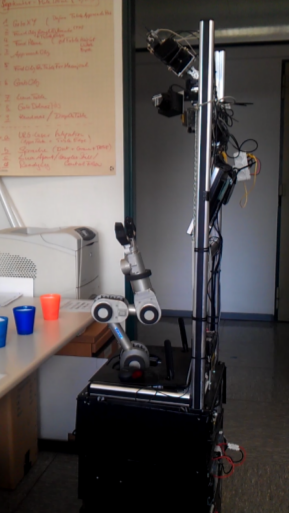
\includegraphics[width=0.7\textwidth]{pics/klingen_real}
    \caption{Grapping a cup in the real scene}
    \label{fig:klingen_real}
  \end{subfigure}
  \begin{subfigure}[b]{0.58\textwidth}
    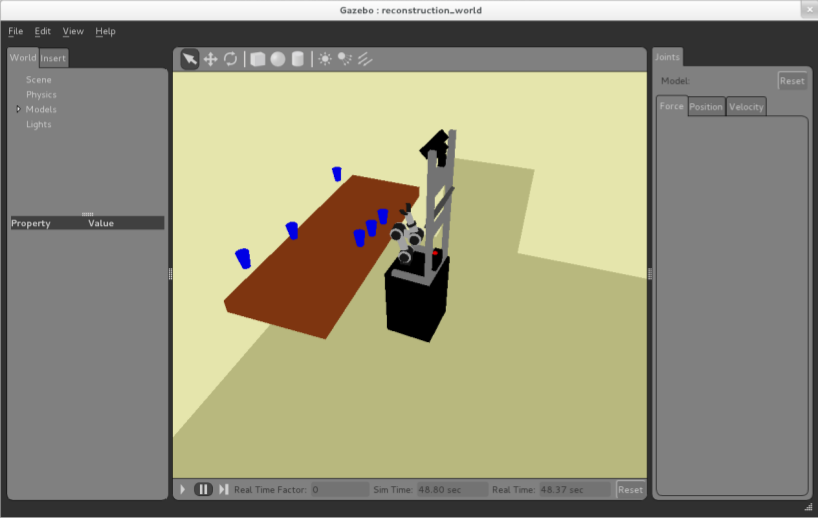
\includegraphics[width=\textwidth]{pics/klingen_sim}
    \caption{Reconstruction in the Gazebo simulator}
    \label{fig:klingen_sim}
  \end{subfigure}
  \caption{Scene Reconstruction for Fault Analysis~\cite{KlingenDA}}
  \label{fig:klingen}
\end{figure}
To establish the communication between Fawkes and Gazebo, Klingen developed a Fawkes plugin that provides the communication objects of the Gazebo \textcolor{red}{API} as an aspect. In this thesis we use this plugin and expend it for our needs. Similar but not so suffisticated as in the thesis by Klingen, we want to provide a possibility to reconstruct faults to find the causes. We do not record the perception of the robots in the simulation but we record the movement of all simulated objects and the high level decisions of the agents which represent can be used to derivate the belief of the robot. The motion of the objects in the simulation can be recorded by Gazebo and the agent decisions by logging our rule-based production system CLIPS. We describe CLIPS in \textcolor{red}{a following section or the background}.

\subsection{Simulation Environment for the Middle Size League}
An other work with Gazebo and Fawkes developed a simulation environment for MSL~\cite{MultiLevelAbstraction}. This simulation environment became necessary because the field size and the amount of robots per team was increased in MSL. Therefore testing became more difficult. The work used an early version of Gazebo and Player as interface between Fawkes and Gazebo. On the one hand, it showed that the Gazebo simulator is capabile of complex components of the robot that cause problems in other simulators. This was shown for omni-directional wheels an an omni-directional camera. \textcolor{red}{Omni-directional wheels can move in one direction similar to normal wheels and have small rolls at the outside of the wheel to be able to move in an other direction without resistance. An omni-directional camera consists of a upwards faced camera and a hyperbolic mirror above, so that the camera can see the whole area around the robot.} Both devices are non-trivial to simulate and often used in MSL. The Robotino we use in this thesis also holds these two devices. On the other hand, the work proposed the idea of multi-level abstraction. If a robot software contains seperate components for steps that are based on each other, it is useful to simulate not only the hardware level, the lowest abstraction level, but also higher abstraction levels. For example if the robot software includes a component that reads an image from a webcam and a component that computes the state of a traffic light from this image, the simulation can provide the simulated image as well as the information about the traffic light. A simulation with multi-level abstraction is able to switch between different abstraction levels. This can be useful to test components on a higher level independent of low level components which can introduce an error or are not finished. Multi-level abstraction has the additional advantage that the components of a higher abstraction level often can be simulated with less computational effort. This makes it easier to run the simulation on a slow computer. However it is not always reasonable to introduce multiple abstraction layers, because some components, such as a collisin avoidance, can not be simulated easily. In this thesis, we also use multi-layer abstraction to be able to test high level components more individually.


\section{Multi-Agent Strategies}
\subsection{Incremental Task-level Reasoning}
Old sim
\subsection{Marked Based Strategies}
